% Chapter 1
\chapter{مقدمه}

\section{شناخت موضوع}

رشد چشمگیر فناوری به همراه سهولت دسترسی به اینترنت در سال‌های اخیر باعث شده که بیشتر دستگاه‌های اطراف خود را متصل به اینترنت ببینیم. این دنیای جدید که به دنیای اینترنت اشیا%
\LTRfootnote{Internet of Things}
معروف است شامل خانه‌های هوشمند%
\LTRfootnote{Smart Homes}%
، دستگاه‌های پوشیدنی%
\LTRfootnote{Wearable Devices}%
، خودروهای خودران و در صدر آن‌ها تلفن‌های هوشمند%
\LTRfootnote{Smart Phones}
است که همگی زندگی روزمره انسان را تغییر داده‌اند. استفاده از این سیستم‌ها همگی باعث تولید حجم قابل توجهی داده در طول روز می‌شوند که شرکت‌های بزرگ فناوری از این داده‌ها بهره برده و با استفاده از آن‌ها اقدام به انواع سرویس‌‌دهی به کاربران خود می‌نمایند.

با توجه به گسترش علم هوش مصنوعی و استفاده از روش‌های یادگیری ماشین، می‌توان از این حجم بسیار زیادِ داده‌ تولید شده به نحو مطلوبی استفاده نمود و الگوریتم‌های مورد نظرمان جهت رسیدن به اهداف مختلف را بر روی آن‌ها اجرا کرد. حال برای مدیریت و اجرای الگوریتم‌های یادگیری، روش‌های مختلفی وجود دارد که به توضیح هر یک از آن‌ها خواهیم پرداخت.

\subsection{یادگیری متمرکز}
روش یادگیری متمرکز%
\LTRfootnote{Centralized Learning}
که در اکثر سیستم‌های حال حاضر امروزی مورد استفاده قرار می‌گیرد به این نحو است که تمام  گره‌ها%
\LTRfootnote{Nodes}
اطلاعات موجود خود را به صورت کامل به سمت سرویس‌دهنده ابری%
\LTRfootnote{Cloud Server}
ارسال می‌نمایند و سرویس‌دهنده ابری در حالی که تمام داده‌ها را در اختیار دارد اقدام به اجرای الگوریتم‌های مورد نظر می‌کند
\cite{elbir2022family}%
. در شکل
\ref{centralized_decentralized_learning}%
(الف) این روش به نمایش گذاشته شده است.

 \begin{figure}[t]
	\centering
	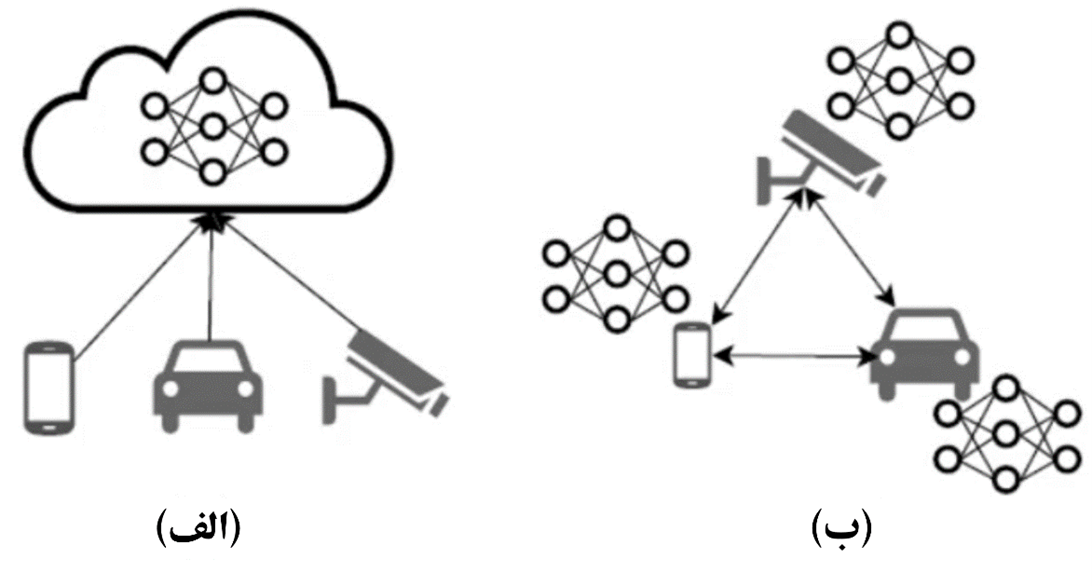
\includegraphics[scale=0.8]{images/chap1/centralized_decentralized_learning.png}%
	\caption{%
(الف) یادگیری متمرکز، (ب) یادگیری غیرمتمرکز
	\cite{zhou2019edge}%
	.
	}
	\label{centralized_decentralized_learning}
	\centering
\end{figure}


\subsection{یادگیری غیر متمرکز}
در روش یادگیری غیر متمرکز%
\LTRfootnote{Decentralized Learning}
هر گره به صورت مجزا اقدام به اجرای الگوریتم‌های مورد نظر می‌کند و در واقع پس از اجرای چند مرحله از کد، اطلاعات به‌روز شده را با گره‌های همسایه به اشتراک می‌گذارد، این کار به قدری ادامه پیدا می‌‎کند تا همگی به مقدار تعیین شده همگرا شوند
\cite{zhou2019edge}%
. در شکل
\ref{centralized_decentralized_learning}%
(ب) این روش به نمایش گذاشته شده است.


\subsection{یادگیری توزیع شده}
روش یادگیری توزیع شده%
\LTRfootnote{Distributed Learning}
به این نحو است که مدیریت کل سیستم و تمام داده‌ها در اختیار یک هسته مرکزی قرار دارد ولی به دلیل نیاز به توان پردازشی بالا، این هسته بار پردازشی را بین گره‌های موجود تقسیم می‌کند. در ابتدای راه یادگیری توزیع‌شده، فرض بر این بوده است که تمام گره‌ها توان پردازشی یکسانی داشته و داده‌ها به میزان مساوی بین گره‌ها پخش خواهند شد. در شکل
\ref{distributed_learning}
این روش به نمایش گذاشته شده است.

 \begin{figure}[t]
	\centering
	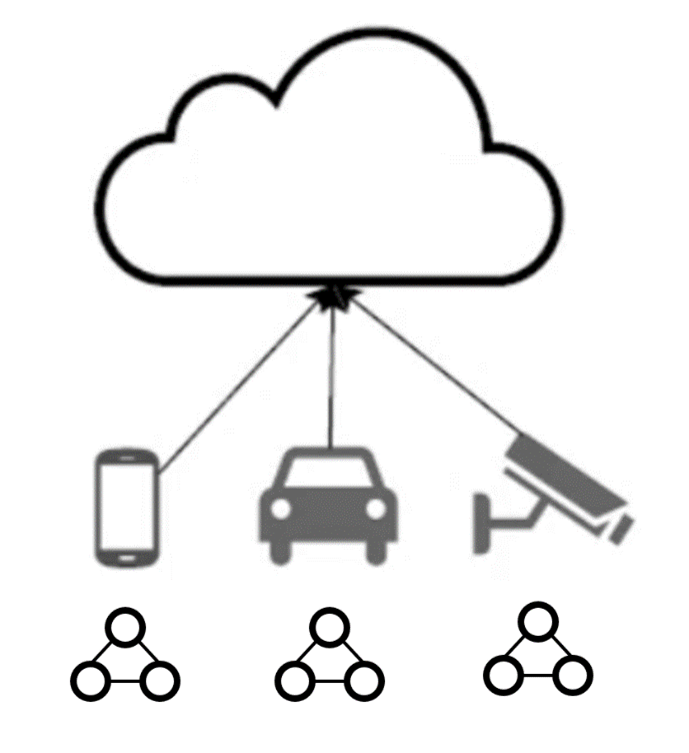
\includegraphics[scale=0.7]{images/chap1/distributed_learning.png}%
	\caption{%
		یادگیری توزیع شده 
		\cite{zhou2019edge}%
		.
	}
	\label{distributed_learning}
	\centering
\end{figure}



\section{یادگیری فدرال}
سیستم‌های متمرکز تا پیش از این، اکثر نیازهای مربوطه را برطرف می‌نمودند ولی در دنیای امروزی و با توجه به زیاد شدن هر روزه دستگاه‌های متصل، موارد دیگری نیز مورد توجه واقع شده است.
هزینه‌های مرتبط با ارسال حجم زیاد داده از یک جهت، و افزایش اضطراب در مورد انتقال اطلاعات حساس و شخصی از حهت دیگر، محققان را به سمت بهره‌گیری از الگوریتم‌های غیرمتمرکز و توزیع شده در زمینه یادگیری ماشین هدایت کرده است.
یکی از زیر مجموعه‌های روش‌های یادگیری توزیع‌شده، شاخه جدید و بسیار پراستفاده یادگیری فدرال بوده که بسیار مورد توجه قرار گرفته است.

در روش یادگیری فدرال، برخلاف رویکردهای متمرکز یادگیری ماشین، تجزیه و تحلیل داده‌ها به دستگاه‌های لبه%
\LTRfootnote{Edge Devices}
یا سرویس‌گیرنده‌ها%
\LTRfootnote{Clients}
منتقل می‌شود. این روش، به عنوان یک جایگزین مطلوب و نوآورانه برای مدل‌سازی داده‌ها در محیط‌هایی با تعداد زیادی سرویس‌گیرنده معرفی شده است. در این چارچوب، به جای انتقال داده‌های اصلی، پارامترهای مدل‌های محلی در هر مرحله از فرآیند آموزش به سمت سرور منتقل می‌شوند، که این امر توانایی بهبود امنیت و کاهش هزینه‌های ارتباطی را فراهم می‌کند.
در شکل
\ref{federated_learning}
این روش به نمایش گذاشته شده است.


 \begin{figure}[t]
	\centering
	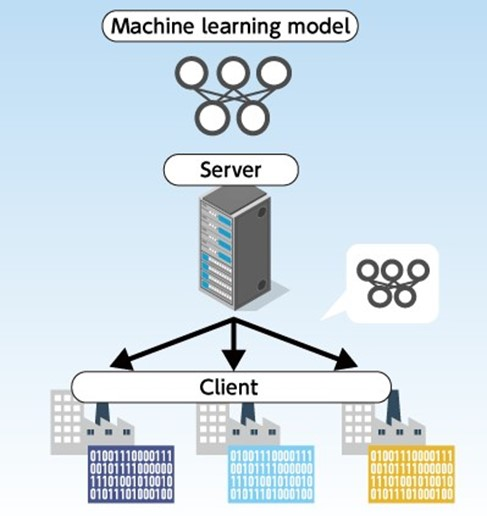
\includegraphics[scale=0.9]{images/chap1/federated_learning.jpg}%
	\caption{%
		یادگیری فدرال 
		\cite{federated_learning}%
		.
	}
	\label{federated_learning}
	\centering
\end{figure}

سرور در حقیقت نقش رهبری را ایفا می‌کند و با توجه به نوع داده‌ها، یک مدل شبکه عصبی%
\LTRfootnote{Neural Network}
ایجاد کرده و آن را به سمت کاربران ارسال می‌کند، حال کاربران با توجه به داده‌های خود شبکه را آموزش می‌دهند و بعد از چند بار تکرار، وزن‌های به‌روزرسانی شده را به سمت سرور بر می‌گردانند. همان‌طور که در شکل
\ref{federated_learning}
مشاهده می‌شود، داده‌ها همگی در سمت کاربران قرار گرفته‌اند و به سمت سرور ارسال نمی‌شوند. عدم اجبار و محدودیت در ارسال اطلاعات گره‌ها در یادگیری فدرال، به حفظ حریم شخصی کاربران کمک می‌کند
\cite{smith2017federated}%
.


\section{تاریخچه یادگیری فدرال}
در ابتدای فصل بهار سال 2017 محققین گوگل
\lr{(Google)}
طی یک مطلب کوتاه در وبلاگ هوش مصنوعی برای اولین بار موضـوع یادگیری فدرال را تحـت مطلبی با عنوان "یادگیری فدرال: یادگیری ماشین اشتـراکی، بدون آموزش متمرکز داده‌ها" مطرح نمودند
\cite{mcmahan2017federated}%
. در این مطلب به طور کوتاه
\lr{Google Keyboard}
یا به اختصار
\lr{Gboard}
معرفی شده و نحوه به کاری‌گیری یادگیری فدرال برای پیش‌بینی لغت بعدی را بیان می‌کند. یادگیری فدرال در این کاربرد نیاز به ارسال داده‌های کاربران به سمت سرور را حذف کرده است و به طور محلی مدل را به‌روزرسانی می‌کند.
بنابراین، با بهره‌گیری از اطلاعات پنهان بسیار زیاد دستگاه‌ها در فرآیند مدل‌سازی، حریم شخصی سرویس‌گیرنده‌ها به نحوی بیشتر از پیش حفظ می‌شود.
در شکل
\ref{gboard}
نحوه استفاده از یادگیری فدرال در این برنامه به نمایش درآمده است.

 \begin{figure}[t]
	\centering
	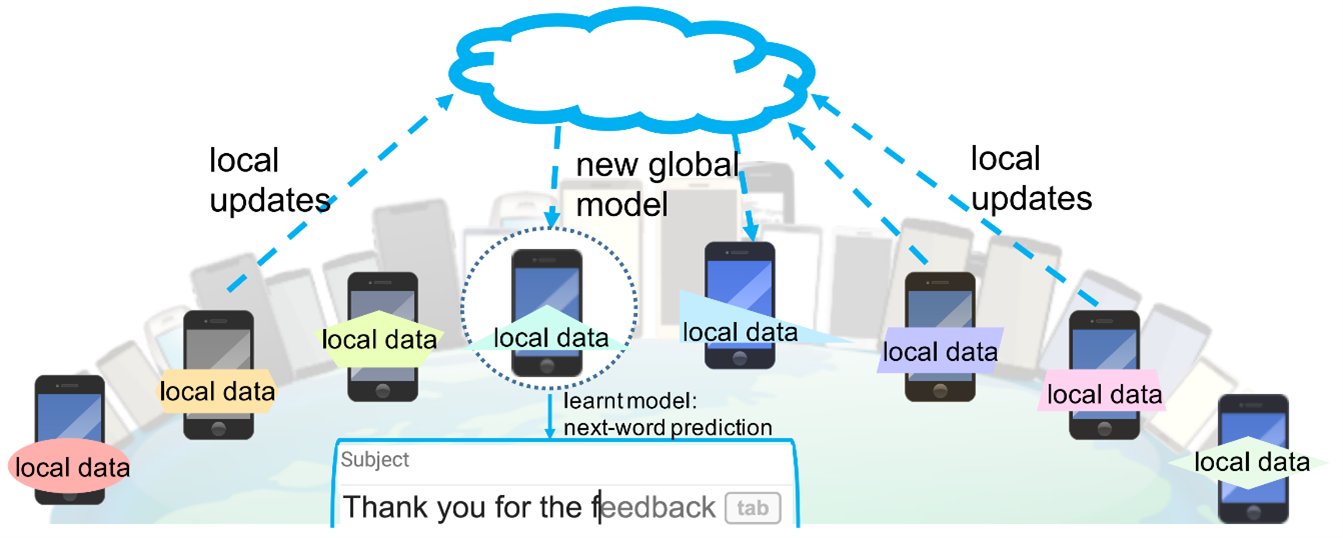
\includegraphics[scale=1]{images/chap1/gboard.png}%
	\caption{%
استفاده از یادگیری فدرال برای پیش‌بینی کلمه بعدی در
\lr{Gboard}
		\cite{li2020federated}%
		.
	}
	\label{gboard}
	\centering
\end{figure}


\section{کاربرد یادگیری فدرال}
تکنولوژی نسل چهار صنعت%
\LTRfootnote{Industry 4.0}%
، دامنه ارتباطات نرم‌افزاری و سخت‌افزاری را در انواع مختلف سیستم‌ها گسترش داده است. این هماهنگی فناوری نرم‌افزار و سخت‌افزار، تبدیل به یک پدیده مهم در مجموعه‌ای از محیط‌های هوشمند و خودکار شده است. سنسورهای سابق که تنها مسئول اندازه‌گیری وضعیت‌ها بودند، جای خود را به دستگاه‌های هوشمند با قابلیت پردازش و برنامه‌ریزی داده‌ها سپرده‌اند. همچنین، گسترش ارتباطات در بستر اینترنت، امکان انتقال و تبادل داده‌ها بین انواع مختلف سیستم‌ها را ارائه کرده است. این پیشرفت‌ها منجر به کاهش نیاز به مرکزیت در تصمیم‌گیری و توسعه سیستم‌ها شده است و به وجود آورنده کنترل و نظارت پیشرفته و توزیع پردازش شده است. این ویژگی‌ها به همراه حجم بی‌سابقه‌ داده، یادگیری فدرال را به یکی از بهترین روش‌های به‌کارگیری در توسعه سیستم‌های هوشمند تبدیل کرده است
\cite{mahtab2022algorithm}%
. در اینجا سه نمونه از کاربرد یادگیری فدرال را شرح خواهیم داد.


\subsection{یادگیری فدرال در شهر هوشمند}
در یک شهر هوشمند%
\LTRfootnote{Smart City}%
، اطلاعات جمع‌آوری شده از سنسورها، دستگاه‌ها و زیرساخت‌های مختلف، از جمله ترافیک، انرژی، پسماند و امنیت، به دلیل ارزش بالایی که دارند، به عنوان منبعی مهم برای بهبود عملکرد و کیفیت زندگی شهروندان محسوب می‌شوند. اما به همراه این ارزش‌ها، حفظ حریم خصوصی و امنیت اطلاعات شهروندان نیز امری بسیار حیاتی است. یادگیری فدرال به عنوان یک رویکرد نوین و مبتنی بر حفظ حریم خصوصی، در اینجا وارد عمل می‌شود.

این روش امکان پردازش داده‌های حساس مانند تصاویر، داده‌های محیطی و اطلاعات مکانی در محیط محلی و توزیع شده را فراهم می‌کند، به‌طوری‌که هر قسمت از شهر می‌تواند به صورت مستقل از سایر قسمت‌ها از این داده‌ها استفاده کند. این رویکرد امکان توسعه مدل‌های هوش مصنوعی و الگوریتم‌های بهبود عملکرد شهر هوشمند را با حفظ حریم خصوصی شهروندان فراهم می‌کند. به‌عنوان مثال، از طریق استفاده از یادگیری فدرال، می‌توان بهبود در مدیریت ترافیک، بهینه‌سازی مصرف انرژی، کاهش آلودگی هوا و افزایش امنیت شهری را به دست آورد، در حالی‌که اطلاعات شخصی شهروندان محافظت می‌شود و از نگرانی‌های حریم خصوصی جلوگیری خواهد شد.


\subsection{یادگیری فدرال در بیمارستان}
در یک بیمارستان، اطلاعات پزشکی بسیار حساس و مهم است که باید محفوظ و محرمانه نگهداری شود. اما در عین حال، استفاده از این داده‌ها برای بهبود خدمات بهداشتی و درمانی نیز بسیار ارزشمند است. در اینجا مفهوم یادگیری فدرال وارد عمل می‌شود. با استفاده از روش‌های یادگیری فدرال، بیمارستان می‌تواند از داده‌های پزشکی بیماران خود برای توسعه مدل‌هایی استفاده کند که پیش‌بینی میزان زمان بستری، بهبود در تشخیص بیماری‌ها و حتی افزایش بهره‌وری پزشکان را ایجاد می‌کنند، بدون اینکه این داده‌ها به‌طور مستقیم در اختیار یک مرکز جمع‌آوری اطلاعات واقع شوند.

به عنوان مثال، با استفاده از یادگیری فدرال، مدل‌های هوش مصنوعی می‌توانند روی داده‌های محلی بیماران بیمارستان‌ها آموزش داده شوند تا بیماری‌های مختلف را شناسایی و تشخیص دهند، و اطلاعات مربوط به درمان‌های مؤثرتر را ارائه دهند، در حالی که اطلاعات حساس بیماران محافظت می‌شود. این روش به بیمارستان‌ها امکان می‌دهد که از داده‌های بیماران خود برای بهبود خدمات بهداشتی و درمانی استفاده کنند، در حالی که رعایت مقررات مربوط به حفظ حریم خصوصی و امنیت داده‌ها را به انجام رسانده‌اند. در شکل
\ref{hospital}
یک نمونه استفاده از یادگیری فدرال در سازمان‌ها به نمایش در آمده است.


\begin{figure}[t]
	\centering
	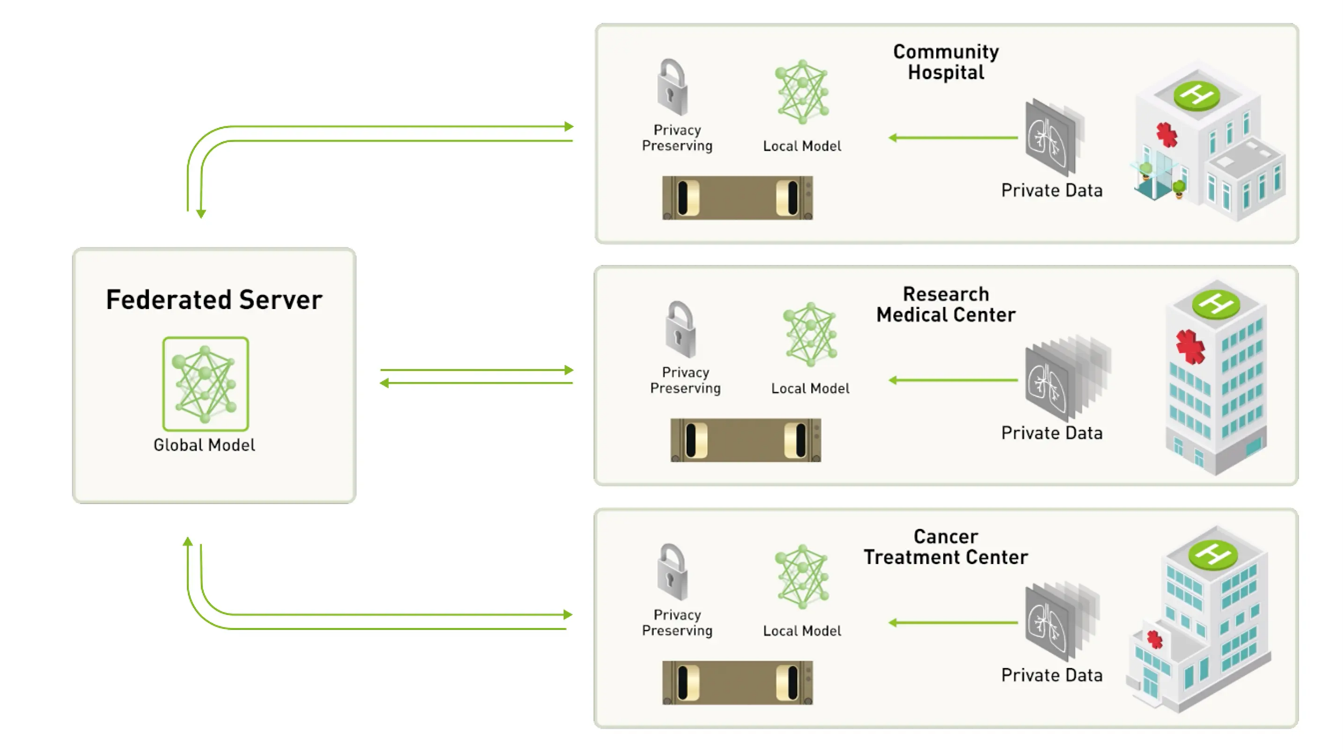
\includegraphics[scale=1]{images/chap1/hospital.png}%
	\caption{%
		یادگیری فدرال در یک بیمارستان
		\cite{kim2012control}%
		.
	}
	\label{hospital}
	\centering
\end{figure}


\subsection{یادگیری فدرال در فروشگاه برنامه‌های کاربردی موبایل}
یک فروشگاه برنامه‌های کاربردی%
\LTRfootnote{App Store}
موبایل را متصور شوید که به کاربران خود امکان می‌دهد برنامه‌های مختلف را دانلود و نصب کنند. این شرکت می‌خواهد با استفاده از داده‌های کاربران خود، الگوریتمی توسعه دهد که به طور دقیق‌تر بتواند پیشنهادات مربوط به برنامه‌هایی که کاربران ممکن است تمایل داشته باشند را ارائه کند.اگر این شرکت از روش‌های متمرکز استفاده کند، باید داده‌های حساس و شخصی کاربران را جمع‌آوری کند و برای آن‌ها تحلیل کند. این ممکن است باعث نگرانی‌های حریم خصوصی کاربران شود و از آن‌ها جلوگیری کند.

در حالی که با استفاده از یادگیری فدرال، این شرکت می‌تواند الگوریتم خود را بر روی داده‌های محلی هر تلفن هوشمند کاربر اجرا کند. به این ترتیب، هیچ داده‌ی حساسی به مرکز جمع‌آوری داده‌ها ارسال نمی‌شود و حریم خصوصی کاربران محفوظ می‌ماند. به عنوان مثال، اگر یک کاربر فقط به برنامه‌های موزیک علاقه‌مند باشد، الگوریتم محلی در تلفن هوشمند او می‌تواند این الگو را تشخیص دهد و پیشنهادات مربوط به برنامه‌های موزیک را به او ارائه دهد، بدون این‌که داده‌های شخصی و حساس او به سرور شرکت ارسال شود. این روش به شرکت امکان می‌دهد از داده‌های کاربران خود برای بهبود خدمات خود استفاده کند، در حالی که حریم خصوصی آن‌ها را محافظت می‌کند.


\section{دید کلی از روند موضوع و بیان هدف پژوهش}
تکمیل این بخش پس از رسیدن به ساختار کلی پایان‌نامه (چون ممکنه در ادامه تغییر کنه)

چند جلمه کلیدی:

به دلیل پراکندگی همگرایی به کندی صورت می‌گیرد

روش جابجایی وزن‌ها بین کاربران نهایی در طول فرایند

چرا جابجایی تصادفی، جابجایی هوشمند بر اساس میزان شباهت

\section{مروی بر روند ارائه مطالب پایان‌نامه}
تست

